\documentclass[11pt,a4paper]{article}
\usepackage[T1]{fontenc}
\usepackage[utf8]{inputenc}
\usepackage[brazil]{babel}
\usepackage{lmodern}
\usepackage[margin=2.2cm]{geometry}
\usepackage{microtype}
\usepackage{graphicx}
\usepackage{float}
\usepackage{booktabs}
\usepackage{array}
\usepackage{adjustbox}
\usepackage{amssymb}
\usepackage[font=small,labelfont=bf]{caption}
\usepackage{fancyvrb}
\usepackage{upquote}
\usepackage{xcolor}
\usepackage{parskip}
\usepackage[colorlinks=true,linkcolor=blue,urlcolor=blue]{hyperref}

% Blocos de saída do notebook e de código para copiar.
\DefineVerbatimEnvironment{saida}{Verbatim}{fontsize=\scriptsize,frame=leftline,framerule=1.5pt,rulecolor=\color{gray!60},xleftmargin=4pt}
\DefineVerbatimEnvironment{codigo}{Verbatim}{fontsize=\footnotesize,frame=single,rulecolor=\color{gray!60}}

% Caixa de destaque para a "ideia central" de cada seção.
\newcommand{\ideia}[1]{\begin{center}\fcolorbox{gray!60}{gray!8}{\parbox{0.94\linewidth}{\small #1}}\end{center}}

\emergencystretch=3em

\title{Etapa 3 --- Construção e avaliação dos classificadores}
\author{Equipe:\\[2pt]
Gabriel Egídio Santos Beloni\\
Gabriel Evangelista Massara\\
Pedro Henrique Cardoso Maia\\
Pedro Tinoco Lanna\\[4pt]
\small Disciplina de Inteligência Artificial --- Profa. Cristiane Neri Nobre\\
\small Trabalho em competição: Detecção de Intrusão em Redes (NSL-KDD)\\[4pt]
\small \textbf{Notebook no Colab:} \href{https://colab.research.google.com/github/pedro-maia1337/IA-CopaLibertadores/blob/main/notebooks/03_modelagem.ipynb}{Abrir o notebook 03 no Google Colab}
% TODO: se gravarem o vídeo da execução, acrescentar a linha abaixo com o link.
% \\\small \textbf{Execução do Notebook:} \href{LINK}{Assistir Vídeo no YouTube}
}
\date{}
\begin{document}
\shorthandoff{"}
\maketitle

\tableofcontents
\clearpage

% =====================================================================
\section*{Resumo dos resultados}
\addcontentsline{toc}{section}{Resumo dos resultados}

Nesta etapa, escolhemos o classificador que vai gerar a submissão da competição. Partimos das melhores configurações de pré-processamento da Etapa 2, comparamos oito algoritmos, ajustamos os hiperparâmetros dos melhores, testamos várias ideias para ganhar alguns décimos de F1-macro e, por fim, congelamos o modelo escolhido em \texttt{results/final\_config.json}. Tudo foi feito só com a base de treino, por validação cruzada agrupada.

\textbf{Sobre a métrica.} Todos os valores deste relatório são F1-macro calculado em \textbf{todas as linhas} de cada fold de validação, como a professora calcula a métrica oficial no teste. A base tem 1.702 grupos de linhas idênticas com rótulos opostos (3.730 linhas). Como a mesma linha recebe uma única previsão, parte dessas cópias sempre erra: nem um classificador perfeito passaria de 0,905, e os bons modelos ficam perto de 0,88. Isso não é falha dos modelos nem vazamento, é aritmética do ruído de rótulo. Na versão anterior deste relatório, o F1-macro era calculado só nas linhas únicas e sem conflito (por isso os valores perto de 0,98); esse número aparece agora apenas como contraste.

\begin{itemize}
\item \textbf{Os ensembles de árvores vencem com folga.} Boosting (HGB, XGBoost) e bagging (Random Forest) ficam entre 0,880 e 0,882 de F1-macro. A rede neural fica em 0,871, e a árvore única e o Naive Bayes ficam bem atrás (0,840 e 0,766).
\item \textbf{Ajustar hiperparâmetros não rendeu.} Os valores padrão já estavam perto do melhor possível. A diferença entre as boas configurações é menor que a variação natural da validação.
\item \textbf{Tentamos subir a nota de cinco formas}: criando atributos novos, fazendo uma busca mais ampla no HGB, testando dois algoritmos de fora da disciplina (LightGBM e CatBoost), tirando a média de várias sementes e combinando modelos por votação. Nenhuma delas superou o melhor modelo único de forma mensurável.
\item \textbf{Modelo escolhido: HGB (Histogram Gradient Boosting)}, com F1-macro de \textbf{0,8819 $\pm$ 0,0030} em validação cruzada repetida 3$\times$5. Uma votação de três modelos (HGB + XGBoost + RF) teve média um pouco maior (0,8826), mas a diferença é quatro vezes menor que a variação entre folds. Pela regra que fixamos antes dos testes, o empate vai para o modelo mais simples.
\item \textbf{Quase todos os erros estão nos conflitos.} Das 1.851 linhas que o HGB erra fora do fold, 1.706 são linhas com rótulo contraditório. No resto da base (66.103 linhas), ele erra 145 e o F1-macro é 0,983. Os erros restantes são, em sua maioria, ataques que se parecem com conexões normais (\texttt{flag=SF}).
\end{itemize}

% =====================================================================
\section*{Como executar o notebook no Google Colab}
\addcontentsline{toc}{section}{Como executar o notebook no Google Colab}

O roteiro é o mesmo das etapas anteriores. A única novidade é que esta etapa usa duas bibliotecas a mais, \texttt{lightgbm} e \texttt{catboost}.

\begin{center}\fbox{\parbox{0.92\linewidth}{\centering\textbf{Repositório a clonar:}\\\url{https://github.com/pedro-maia1337/IA-CopaLibertadores.git}}}\end{center}

\begin{enumerate}
\item \textbf{Abra o notebook} pelo \href{https://colab.research.google.com/github/pedro-maia1337/IA-CopaLibertadores/blob/main/notebooks/03_modelagem.ipynb}{link direto} ou por \textbf{Arquivo > Abrir notebook > GitHub}, escolhendo \texttt{notebooks/03\_modelagem.ipynb}.
\item \textbf{Envie o \texttt{treino.csv}} para \texttt{/content} pelo painel \textbf{Arquivos} do Colab. Esta etapa também não usa o teste.
\item \textbf{Prepare o ambiente} com uma célula no topo do notebook. Nenhuma linha tem recuo, então o trecho funciona mesmo copiado do PDF, que costuma perder os espaços do começo das linhas:
\end{enumerate}

\begin{codigo}
import sys
REPO = "/content/IA-CopaLibertadores"
!test -d {REPO} || git clone https://github.com/pedro-maia1337/IA-CopaLibertadores.git {REPO}
%cd {REPO}
!pip install -q "scikit-learn>=1.6" "imbalanced-learn>=0.12" "xgboost>=2.1"
!pip install -q "lightgbm>=4.5" "catboost>=1.2" "shap>=0.46" "seaborn>=0.13"
!mkdir -p data/new-database
!cp /content/treino.csv data/new-database/
sys.path.insert(0, f"{REPO}/src")
\end{codigo}

\begin{enumerate}\setcounter{enumi}{3}
\item \textbf{Execute tudo} (\textbf{Ambiente de execução > Executar tudo}). Se o \texttt{pip} atualizar o numpy ou o pandas, reinicie a sessão e execute de novo.
\end{enumerate}

\textbf{Tempo de execução.} Para ver os resultados, não é preciso executar nada: o notebook entregue já está executado, com todas as tabelas e figuras salvas. Se quiser reexecutá-lo, ele leva \textbf{poucos minutos}. A Etapa 3 avalia 135 configurações, cada uma com uma validação cruzada completa, e calcular tudo do zero leva cerca de 2 horas no nosso computador (16 núcleos). Para não repetir esse trabalho, cada resultado fica guardado em \texttt{results/experiments.csv}, que vem junto com o repositório, e o notebook só lê o que já foi calculado. Cada resultado é identificado por uma etiqueta montada a partir dos parâmetros do experimento. Como uma versão diferente das bibliotecas pode acrescentar parâmetros novos ao modelo e mudar essa etiqueta, cada resultado tem também uma etiqueta \emph{estável}, que considera só os parâmetros que escolhemos (os diferentes do padrão). Assim, o registro é encontrado mesmo com as versões do Colab, e o notebook avisa quando isso acontece. Quem quiser refazer todos os cálculos pode mudar \texttt{RECALCULAR = False} para \texttt{True} na primeira célula de código; com os 2 núcleos do Colab gratuito, isso pode levar muitas horas.

% =====================================================================
\setcounter{section}{-1}
\section{Configuração e regras sobre os dados}

Usamos a mesma semente (\texttt{RANDOM\_STATE = 42}), a mesma versão da base (\texttt{db8fb3ac}) e o mesmo registro de experimentos das etapas anteriores. A primeira célula do notebook mostra as versões das bibliotecas e o tamanho da base:

\begin{saida}
{'numpy': '2.5.4', 'pandas': '3.0.6', 'sklearn': '1.9.1', 'imblearn': '0.14.2',
 'xgboost': '3.4.1', 'lightgbm': '4.7.0', 'catboost': '1.2.10'}
RANDOM_STATE = 42 | versão da base: db8fb3ac
X: (69833, 41) | classes: {'normal': 65754, 'anomaly': 4079}
\end{saida}

As regras sobre os dados também não mudaram:

\begin{itemize}
\item \textbf{Só o treino é usado.} O \texttt{teste\_sem\_rotulo.csv} só será aberto no notebook 04, uma única vez, depois do congelamento do modelo. A base original do NSL-KDD (\texttt{data/raw/}) não é usada, porque contém as linhas do teste com os rótulos.
\item \textbf{Só os 41 atributos de rede entram no modelo.} As três colunas de vazamento (\texttt{score\_ids\_legado}, \texttt{tipo\_alerta\_soc} e \texttt{tempo\_resposta\_analista\_min}) e as cinco cópias derivadas ficam de fora.
\item \textbf{Tudo que aprende com os dados fica dentro do pipeline.} Limpeza de rótulos, imputação, codificação, escala e seleção são passos do \texttt{Pipeline}. A validação cruzada recebe o pipeline inteiro, então cada passo é ajustado só com os folds de treino. O limiar de decisão também é escolhido só com previsões feitas fora do fold.
\end{itemize}

% =====================================================================
\section{Como comparamos os modelos}

\ideia{\textbf{Ideia central:} medir todos os modelos do mesmo jeito, numa régua que imite o teste, e decidir \emph{antes} de ver os resultados como o vencedor seria escolhido.}

\textbf{Validação cruzada agrupada.} A base tem muitas linhas repetidas. Se uma cópia ficasse no treino e outra na validação, o modelo seria testado em algo que já viu, e a nota sairia inflada. Por isso, usamos \texttt{StratifiedGroupKFold} com 5 folds: todas as cópias de uma mesma linha ficam sempre do mesmo lado.

\textbf{Métrica.} Usamos o F1-macro, que é a métrica oficial da competição. Ele é a média do F1 das duas classes, então a classe minoritária (\texttt{anomaly}) pesa tanto quanto a majoritária. Pontuamos cada fold em \textbf{todas as linhas}, com cópias e conflitos, porque é assim que a métrica oficial é calculada no teste. Nos 1.702 grupos em que a mesma linha aparece com os dois rótulos, o modelo dá uma única resposta, e parte das cópias sempre erra. Por isso, mesmo um classificador perfeito fora dos conflitos, que escolhesse o melhor rótulo em cada conflito, ficaria em 0,905. Como contraste, registramos também o F1-macro do mesmo modelo, com o mesmo limiar, só nas linhas únicas e sem conflito. Esse valor mostra quanto do erro vem do ruído de rótulo, mas não decide nada e não estima a nota.

\textbf{Por que não a acurácia.} Há 16 conexões normais para cada ataque. Um ``modelo'' que responde sempre \texttt{normal} já tem 94\% de acurácia, mas F1-macro de apenas 0,48. A acurácia aparece nas tabelas só para mostrar o quanto ela engana.

\textbf{Limiar de decisão.} O modelo devolve uma probabilidade de ataque, e precisamos de um ponto de corte para transformá-la em \texttt{normal} ou \texttt{anomaly}. O corte padrão é 0,5, mas, com a classe de ataque tão minoritária, um corte mais baixo costuma dar F1-macro maior. Escolhemos o corte com previsões feitas \emph{fora} do fold que está sendo pontuado, para que ele nunca ajude a escolher o próprio limiar. No modelo final, o \texttt{ThresholdClassifier} faz o mesmo dentro do treino.

\textbf{Pré-processamento.} Cada algoritmo recebe a configuração que venceu na Etapa 2 para a sua família:
\begin{itemize}
\item \textbf{Boosting} (HGB, XGBoost, LightGBM, CatBoost): remoção dos grupos com rótulo contraditório no treino de cada fold (\texttt{drop\_inconsistent}), valores ausentes e categorias tratados pelo próprio algoritmo, sem escala.
\item \textbf{Bagging e árvore única} (RF, Extra Trees, DT): imputação pela mediana e one-hot nas categorias, sem redução.
\item \textbf{Modelos sensíveis a escala} (MLP, KNN, Naive Bayes): mediana, one-hot, \texttt{log1p} e padronização. O KNN usa também a seleção dos 30 melhores atributos.
\end{itemize}

\textbf{Regra de escolha, fixada antes dos resultados.}
\begin{enumerate}
\item Vence o maior F1-macro médio na validação cruzada \textbf{repetida 3$\times$5} (três sorteios diferentes dos 5 folds, 15 medições ao todo).
\item Uma diferença menor que 1 desvio-padrão entre folds conta como \textbf{empate}.
\item No empate, vence o modelo \textbf{mais simples e explicável}: menos modelos para treinar, menos passos no pipeline e, por último, algoritmo visto na disciplina.
\end{enumerate}

A regra protege contra um erro comum em competições: com dezenas de candidatos e diferenças minúsculas, o primeiro colocado na validação muitas vezes é só o que teve mais sorte na divisão dos folds.

% =====================================================================
\section{Comparação de oito algoritmos}

\ideia{\textbf{Ideia central:} antes de ajustar qualquer coisa, ver qual família de algoritmos se dá melhor com estes dados.}

Testamos oito algoritmos, cobrindo as famílias vistas na disciplina, todos com hiperparâmetros padrão razoáveis e validação agrupada de 5 folds.

\begin{figure}[H]
\centering
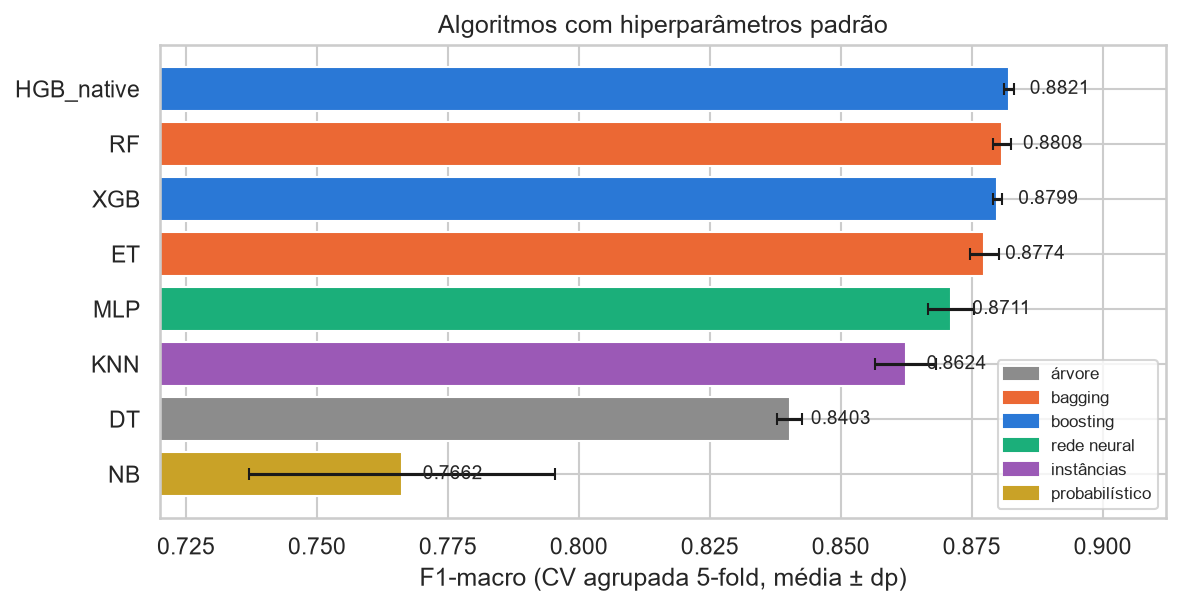
\includegraphics[width=\linewidth,height=0.30\textheight,keepaspectratio]{figuras/mod_algoritmos.png}
\caption{F1-macro de cada algoritmo com hiperparâmetros padrão. A barra preta mostra $\pm$1 desvio-padrão entre os folds.}
\end{figure}

\begin{table}[H]
\centering
\caption{Os oito algoritmos com hiperparâmetros padrão (CV agrupada, 5 folds, todas as linhas). Precisão e recall de \texttt{anomaly} ficam perto de 0,75--0,80 porque metade das cópias em conflito é rotulada \texttt{anomaly}.}
\label{tab:algoritmos}
\begin{adjustbox}{max width=\linewidth}
\begin{tabular}{llrrrrrrr}
\toprule
Algoritmo & Família & F1-macro & dp & F1 anomaly & precisão anomaly & recall anomaly & acurácia & tempo (s) \\
\midrule
HGB & boosting & \textbf{0.8821} & 0.0009 & 0.7784 & 0.7565 & 0.8017 & 0.9733 & 14 \\
Random Forest & bagging & 0.8808 & 0.0018 & 0.7760 & 0.7534 & 0.8002 & 0.9730 & 33 \\
XGBoost & boosting & 0.8799 & 0.0008 & 0.7742 & 0.7506 & 0.7995 & 0.9728 & 16 \\
Extra Trees & bagging & 0.8774 & 0.0028 & 0.7695 & 0.7539 & 0.7857 & 0.9725 & 43 \\
MLP & rede neural & 0.8711 & 0.0044 & 0.7576 & 0.7456 & 0.7705 & 0.9712 & 24 \\
KNN & instâncias & 0.8624 & 0.0058 & 0.7410 & 0.7352 & 0.7472 & 0.9695 & 13 \\
Árvore de Decisão & árvore única & 0.8403 & 0.0024 & 0.7015 & 0.6333 & 0.7867 & 0.9609 & 15 \\
Naive Bayes & probabilístico & 0.7662 & 0.0292 & 0.5696 & 0.4596 & 0.7578 & 0.9318 & 11 \\
\bottomrule
\end{tabular}
\end{adjustbox}
\end{table}

\textbf{O que os resultados mostram.}
\begin{itemize}
\item \textbf{Os ensembles de árvores dominam.} HGB, Random Forest e XGBoost ficam praticamente empatados no topo. Os atributos do KDD são contagens e taxas com fronteiras nítidas: por exemplo, uma taxa alta de erros SYN (\texttt{serror\_rate}) indica uma varredura de portas. Cortes do tipo ``\texttt{serror\_rate} $>$ 0,8'' são exatamente o que uma árvore aprende.
\item \textbf{A árvore única perde 4 pontos}, muito numa escala em que o teto é 0,905. Sozinha, ela se ajusta demais aos exemplos com rótulo errado. Os ensembles corrigem isso: o bagging tira a média de muitas árvores, e o boosting corrige os erros de uma árvore com a seguinte. Note que a árvore única tem 96,1\% de acurácia, mas acerta só 63\% das vezes em que acusa um ataque. A acurácia esconde esse problema, e o F1-macro o mostra.
\item \textbf{MLP e KNN ficam no meio.} Os dois dependem de distâncias e de escala. Mesmo com \texttt{log1p} e padronização, a mistura de dezenas de colunas one-hot de \texttt{service} com taxas contínuas atrapalha.
\item \textbf{O Naive Bayes é o pior e o mais instável.} Ele supõe que os atributos são independentes entre si, mas muitas taxas do KDD andam juntas (\texttt{serror\_rate}, \texttt{srv\_serror\_rate}, \texttt{dst\_host\_serror\_rate}). Ele acaba contando a mesma evidência várias vezes e dispara alarmes demais (precisão de 46\%).
\end{itemize}

Seguiram para o ajuste de hiperparâmetros os três melhores (HGB, RF e XGBoost) e o MLP, que representa as redes neurais citadas no enunciado.

% =====================================================================
\section{Ajuste de hiperparâmetros}

\ideia{\textbf{Ideia central:} procurar configurações melhores que o padrão usando a mesma régua de antes.}

Fizemos uma busca aleatória: sorteamos de 6 a 12 combinações de hiperparâmetros por algoritmo e avaliamos cada uma com a mesma validação agrupada. Não usamos o \texttt{GridSearchCV} pronto do scikit-learn porque ele não escolhe o limiar fora do fold.

\begin{figure}[H]
\centering
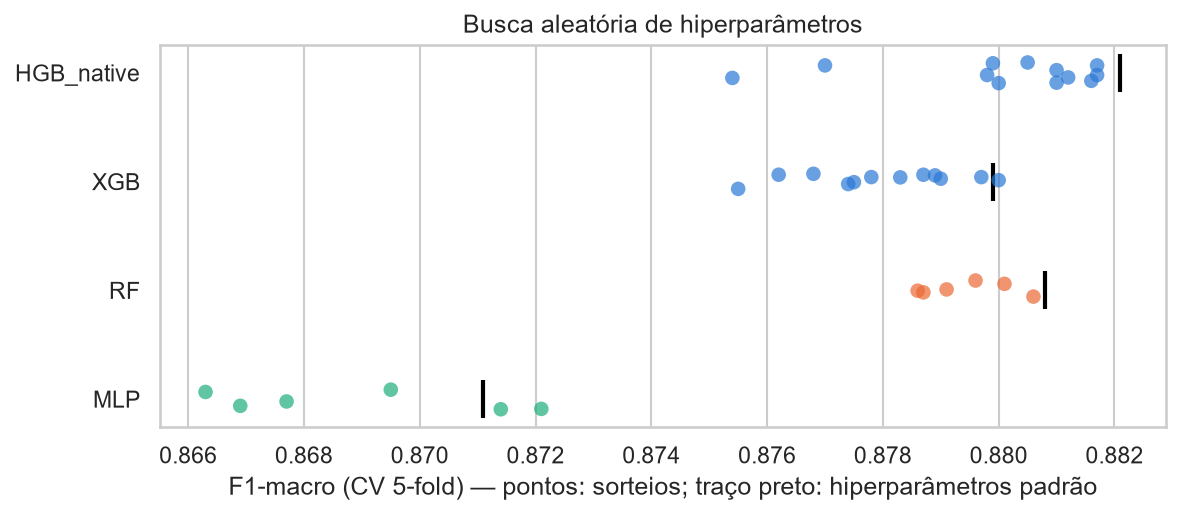
\includegraphics[width=\linewidth,height=0.30\textheight,keepaspectratio]{figuras/mod_busca.png}
\caption{Cada ponto é uma combinação sorteada; a linha marca o resultado com os valores padrão.}
\end{figure}

\begin{table}[H]
\centering
\caption{Valores padrão contra o melhor sorteio da busca (CV agrupada, 5 folds).}
\begin{tabular}{lrrr}
\toprule
Algoritmo & sorteios & F1 padrão & F1 melhor sorteio \\
\midrule
HGB & 12 & 0.8821 & 0.8817 \\
Random Forest & 6 & 0.8808 & 0.8806 \\
XGBoost & 12 & 0.8799 & 0.8800 \\
MLP & 6 & 0.8711 & 0.8721 \\
\bottomrule
\end{tabular}
\end{table}

\textbf{O que os resultados mostram.} A busca não encontrou nada melhor que o padrão. No HGB, o melhor sorteio ficou até um pouco abaixo; nos demais, a diferença está dentro do ruído. Os valores padrão desses algoritmos já são escolhas consagradas, e a base é ``fácil'' para eles. A busca mostrou que os hiperparâmetros importam para fugir de configurações ruins (no HGB, os sorteios variam até 0,006), mas não separam as configurações boas entre si.

% =====================================================================
\section{Tentativas de ganho adicional}

\ideia{\textbf{Ideia central:} como é uma competição, testamos várias ideias para subir alguns décimos, sempre sem tocar no teste e sempre dentro do pipeline.}

\subsection{Atributos novos}

Criamos 12 atributos calculados a partir de cada linha, como razões e produtos. Um exemplo: as taxas do KDD perdem a escala. ``100\% de erros SYN'' em 2 conexões e em 500 conexões são situações muito diferentes, mas a taxa é a mesma. Multiplicar a taxa pela contagem (\texttt{serror\_count}) entrega essa informação pronta para a árvore. Como cada atributo usa só a própria linha e uma fórmula fixa, aplicá-lo ao teste não usa nenhuma informação do teste.

\begin{table}[H]
\centering
\caption{Efeito dos atributos novos (CV agrupada, 5 folds).}
\begin{tabular}{lrrr}
\toprule
Algoritmo & sem atributos & com atributos & diferença \\
\midrule
HGB & 0.8817 & 0.8808 & $-$0.0009 \\
XGBoost & 0.8800 & 0.8783 & $-$0.0017 \\
Random Forest & 0.8806 & 0.8805 & $-$0.0001 \\
\bottomrule
\end{tabular}
\end{table}

Nenhum modelo melhorou: os três ficaram iguais ou um pouco piores. As árvores já conseguiam combinar taxa e contagem sozinhas, e as colunas redundantes diluem a amostragem de atributos do XGBoost e do RF. A ideia ainda passou pela validação repetida (Seção~\ref{sec:finalistas}), para não ser descartada por causa de uma única divisão dos folds.

\subsection{Busca mais ampla no HGB}

O HGB é o melhor modelo e também o mais rápido (cerca de 15 segundos por validação). Isso permitiu uma segunda busca, com 20 sorteios num espaço mais largo: mais iterações, árvores maiores e amostragem de colunas.

\begin{figure}[H]
\centering
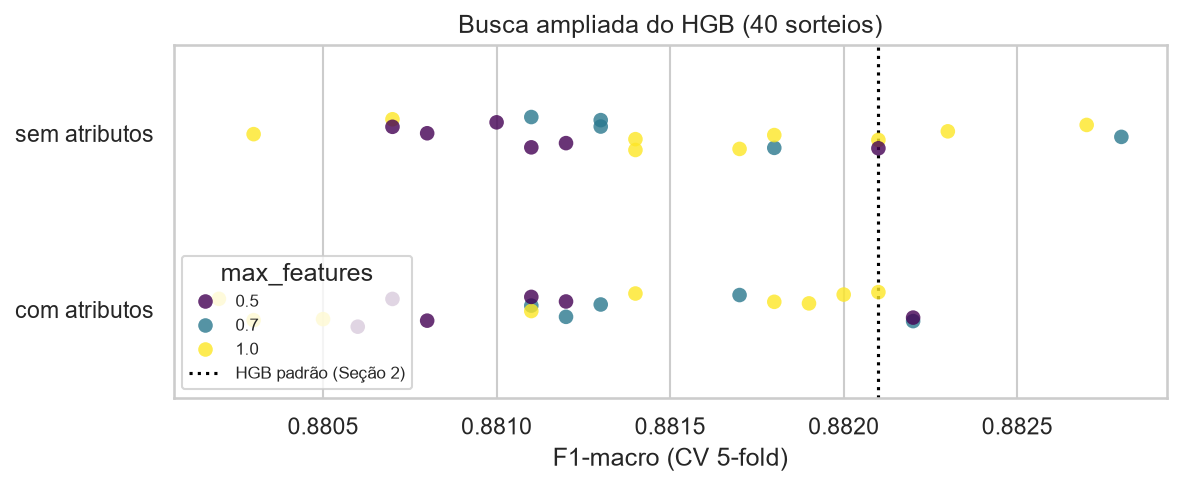
\includegraphics[width=\linewidth,height=0.28\textheight,keepaspectratio]{figuras/mod_busca_hgb2.png}
\caption{Segunda busca no HGB, sem e com os atributos novos.}
\end{figure}

O melhor sorteio chegou a 0,8828, com folhas de no mínimo 20 exemplos (mais regularização), taxa de aprendizado de 0,08 e 70\% das colunas por iteração. A maioria dos sorteios, porém, ficou abaixo do HGB padrão (a média é 0,8815, contra 0,8821). Quando se escolhe o melhor de 20 tentativas, parte do ganho é sorte. Por isso, o vencedor da busca também passou pela validação repetida.

\subsection{Algoritmos de fora da disciplina: LightGBM e CatBoost}

O enunciado exige ao menos três algoritmos vistos na disciplina, requisito já cumprido, mas não proíbe outros. Testamos os dois algoritmos de boosting mais usados em competições de dados tabulares:
\begin{itemize}
\item \textbf{LightGBM}: muito parecido com o HGB, mas cresce cada árvore pela folha que mais reduz o erro, em vez de nível por nível.
\item \textbf{CatBoost}: usa árvores ``simétricas'', em que todos os nós de um mesmo nível fazem o mesmo corte, e codifica as categorias com estatísticas do rótulo calculadas de forma ordenada.
\end{itemize}

Os dois receberam o mesmo pré-processamento do HGB e passaram pelo mesmo protocolo: valores padrão primeiro e depois uma busca aleatória.

\begin{table}[H]
\centering
\caption{LightGBM e CatBoost (CV agrupada, 5 folds).}
\begin{tabular}{lrrr}
\toprule
Algoritmo & sorteios & F1 padrão & F1 melhor sorteio \\
\midrule
LightGBM & 20 & 0.8818 & 0.8822 \\
CatBoost & 8 & 0.8760 & 0.8777 \\
\bottomrule
\end{tabular}
\end{table}

O LightGBM empatou com o HGB, o que é esperado, já que os dois funcionam de forma muito parecida. O CatBoost ficou atrás e é cerca de 5 vezes mais lento. Ter o mesmo corte em todo um nível regulariza bem bases pequenas, mas dificulta aprender regras muito específicas, como as que separam ataques raros.

\subsection{Média de sementes e votação}

Também testamos duas formas de combinar modelos, avaliadas na Seção~\ref{sec:finalistas}:
\begin{itemize}
\item \textbf{Média de 5 sementes}: o mesmo HGB treinado 5 vezes, cada vez com uma amostra diferente de colunas, e a média das 5 probabilidades.
\item \textbf{Votação suave}: a média das probabilidades de modelos diferentes (HGB + RF + XGBoost, HGB + LightGBM, HGB + CatBoost e HGB + LightGBM + CatBoost).
\end{itemize}

% =====================================================================
\section{Finalistas em validação repetida (3$\times$5)}
\label{sec:finalistas}

\ideia{\textbf{Ideia central:} com diferenças tão pequenas, uma única validação não basta. Repetimos a validação três vezes, com divisões diferentes, para separar ganho real de sorte.}

Uma validação de 5 folds tem desvio-padrão de 0,001 a 0,003, da mesma ordem das diferenças entre os candidatos. Por isso, os 15 finalistas foram reavaliados com a validação agrupada repetida 3 vezes (sementes 42, 43 e 44, 15 folds ao todo). É essa medida que decide.

\begin{figure}[H]
\centering
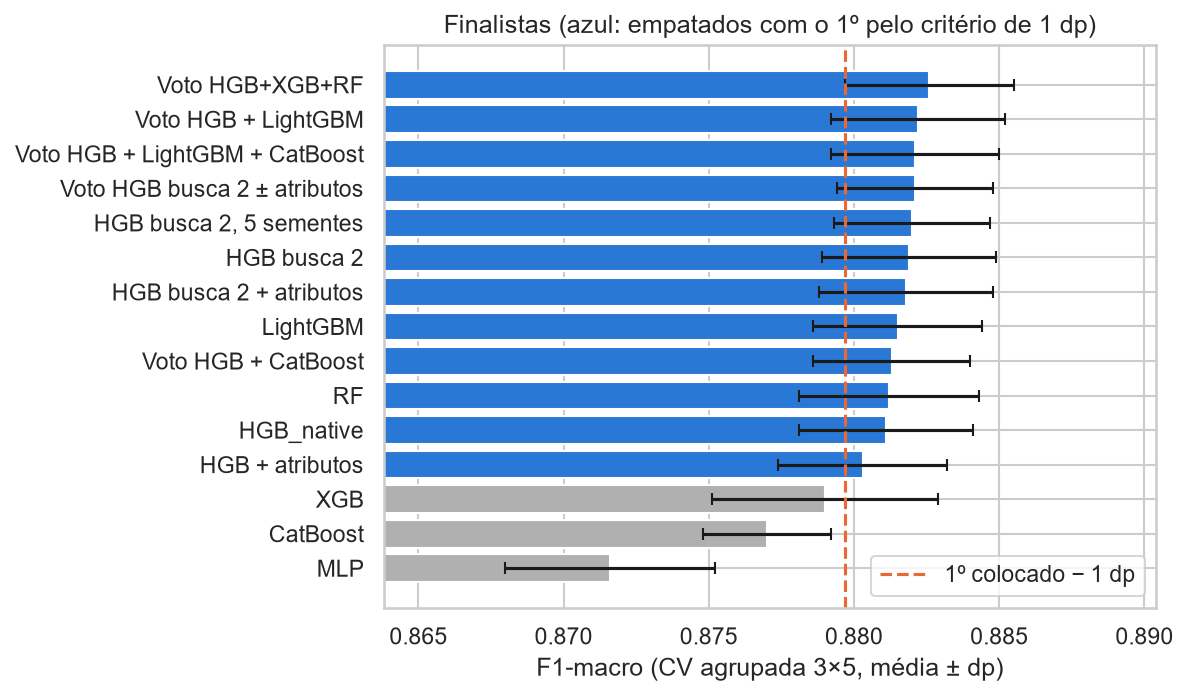
\includegraphics[width=0.9\linewidth,height=0.36\textheight,keepaspectratio]{figuras/mod_finalistas.png}
\caption{Os 15 finalistas. Em azul, os que estão a menos de 1 desvio-padrão do primeiro colocado, ou seja, empatados com ele. A linha tracejada marca esse limite.}
\end{figure}

\begin{table}[H]
\centering
\caption{Finalistas em CV agrupada 3$\times$5, ordenados pelo F1-macro (todas as linhas). A coluna ``sem conflitos'' é o contraste: o mesmo modelo e limiar, só nas linhas únicas e sem rótulo contraditório. A última coluna indica empate com o 1º colocado (diferença menor que 1 dp).}
\label{tab:finalistas}
\begin{adjustbox}{max width=\linewidth}
\begin{tabular}{lrrrrrrrc}
\toprule
Modelo & F1-macro & dp & sem conflitos & F1 anomaly & precisão anomaly & recall anomaly & tempo (s) & empata? \\
\midrule
Voto HGB + XGBoost + RF & 0.8826 & 0.0029 & 0.9821 & 0.7794 & 0.7568 & 0.8035 & 663 & 1º \\
Voto HGB + LightGBM & 0.8822 & 0.0030 & 0.9821 & 0.7786 & 0.7587 & 0.7996 & 138 & \checkmark \\
Voto HGB busca 2 $\pm$ atributos & 0.8821 & 0.0027 & 0.9821 & 0.7783 & 0.7584 & 0.7993 & 117 & \checkmark \\
Voto HGB + LightGBM + CatBoost & 0.8821 & 0.0029 & 0.9820 & 0.7784 & 0.7588 & 0.7991 & 276 & \checkmark \\
HGB busca 2, 5 sementes & 0.8820 & 0.0027 & 0.9819 & 0.7782 & 0.7588 & 0.7987 & 224 & \checkmark \\
\textbf{HGB busca 2 (escolhido)} & \textbf{0.8819} & 0.0030 & 0.9817 & 0.7779 & 0.7588 & 0.7982 & 76 & \checkmark \\
HGB busca 2 + atributos & 0.8818 & 0.0030 & 0.9819 & 0.7777 & 0.7589 & 0.7976 & 77 & \checkmark \\
LightGBM & 0.8815 & 0.0029 & 0.9812 & 0.7772 & 0.7589 & 0.7965 & 63 & \checkmark \\
Voto HGB + CatBoost & 0.8813 & 0.0027 & 0.9812 & 0.7767 & 0.7594 & 0.7950 & 326 & \checkmark \\
Random Forest & 0.8812 & 0.0031 & 0.9801 & 0.7768 & 0.7551 & 0.7999 & 619 & \checkmark \\
HGB (1ª busca) & 0.8811 & 0.0030 & 0.9791 & 0.7764 & 0.7534 & 0.8011 & 71 & \checkmark \\
HGB + atributos & 0.8803 & 0.0029 & 0.9787 & 0.7749 & 0.7552 & 0.7959 & 85 & \checkmark \\
XGBoost & 0.8790 & 0.0039 & 0.9769 & 0.7725 & 0.7549 & 0.7910 & 68 & \\
CatBoost & 0.8770 & 0.0022 & 0.9739 & 0.7686 & 0.7531 & 0.7849 & 289 & \\
MLP & 0.8716 & 0.0036 & 0.9625 & 0.7587 & 0.7362 & 0.7830 & 165 & \\
\bottomrule
\end{tabular}
\end{adjustbox}
\end{table}

\textbf{O que os resultados mostram.}
\begin{itemize}
\item \textbf{Onze candidatos empatam com o primeiro.} A votação HGB + XGBoost + RF tem a maior média (0,8826), mas o HGB da busca ampliada fica a 0,0007 dela, quatro vezes menos que o desvio entre folds.
\item \textbf{Combinar modelos não ajudou.} Média de sementes, votações entre HGBs e votações com outros algoritmos ficam todas dentro da variação do modelo único. A votação só corrige erros quando os modelos erram em exemplos \emph{diferentes}. Aqui, os modelos fortes erram quase sempre nos mesmos (Seção~\ref{sec:erros}).
\item \textbf{Os atributos novos não se confirmaram.} Na validação repetida, o HGB com atributos (0,8803) ficou abaixo do HGB sem eles (0,8811), e na busca ampliada os dois empatam (0,8818 e 0,8819).
\item \textbf{O LightGBM alcança o HGB, mas não o supera.} O CatBoost e o XGBoost ficam fora do empate.
\item \textbf{A coluna sem conflitos conta a mesma história em outra escala.} Sem as linhas contraditórias, os mesmos modelos ficam entre 0,96 e 0,98, quase na mesma ordem. A distância para os 0,88 da métrica oficial é o efeito dos conflitos, igual para todos os modelos.
\end{itemize}

% =====================================================================
\section{Tabela comparativa consolidada}

As Tabelas~\ref{tab:algoritmos} e~\ref{tab:finalistas} são a tabela comparativa pedida no enunciado: cada linha combina um algoritmo com o pré-processamento da sua família, e as colunas trazem as métricas da validação agrupada. As versões completas, com todas as colunas, estão em \texttt{results/tabela\_etapa3\_algoritmos.csv} e \texttt{results/tabela\_etapa3\_finalistas.csv}. Abaixo, resumimos qual pré-processamento ajuda qual algoritmo, e por quê.

\begin{table}[H]
\centering
\caption{Qual pré-processamento ajuda qual algoritmo.}
\begin{adjustbox}{max width=\linewidth}
\begin{tabular}{p{3.4cm}p{3.6cm}p{9.4cm}}
\toprule
Técnica & Quem ganha & Por quê \\
\midrule
Limpeza de rótulos (\texttt{drop\_inconsistent}) & boosting (HGB: +0,004 na Etapa 2) & O boosting ajusta cada árvore aos erros da anterior e acaba ``perseguindo'' exemplos com rótulo trocado. O bagging tira a média de muitas árvores, o que já dilui esse ruído. \\
\texttt{log1p} + padronização & MLP e KNN & Esses modelos usam distâncias e gradientes, e as caudas longas de \texttt{src\_bytes} e \texttt{dst\_bytes} dominariam o cálculo. As árvores só olham a ordem dos valores, então não mudam. \\
Categorias nativas & HGB, LightGBM, CatBoost & O próprio algoritmo agrupa vários serviços num só corte. Os demais usam one-hot, que não cria uma ordem falsa entre os serviços. \\
NaN nativo & HGB, XGBoost, LightGBM & O algoritmo aprende para que lado da divisão mandar o valor ausente. Os demais precisam de imputação pela mediana. \\
Seleção de atributos & KNN (30 melhores) & No KNN, tira do cálculo das distâncias dimensões que só atrapalham. No RF, a seleção por árvores empatou com não reduzir (Etapa 2). O PCA perdeu em todos os testes. \\
Balanceamento & nenhum & O limiar de decisão ajustado (entre 0,04 e 0,36 nos finalistas) já compensa o desbalanceamento, sem criar exemplos sintéticos. \\
\bottomrule
\end{tabular}
\end{adjustbox}
\end{table}

% =====================================================================
\section{Onde o modelo escolhido erra}
\label{sec:erros}

\ideia{\textbf{Ideia central:} olhar os erros mostra se ainda há algo a corrigir ou se chegamos ao limite dos dados. Esta análise é só diagnóstica e não mudou nenhuma escolha.}

Usamos previsões feitas fora do fold (cada linha é prevista por um modelo que não a viu no treino) com o HGB escolhido.

\begin{figure}[H]
\centering
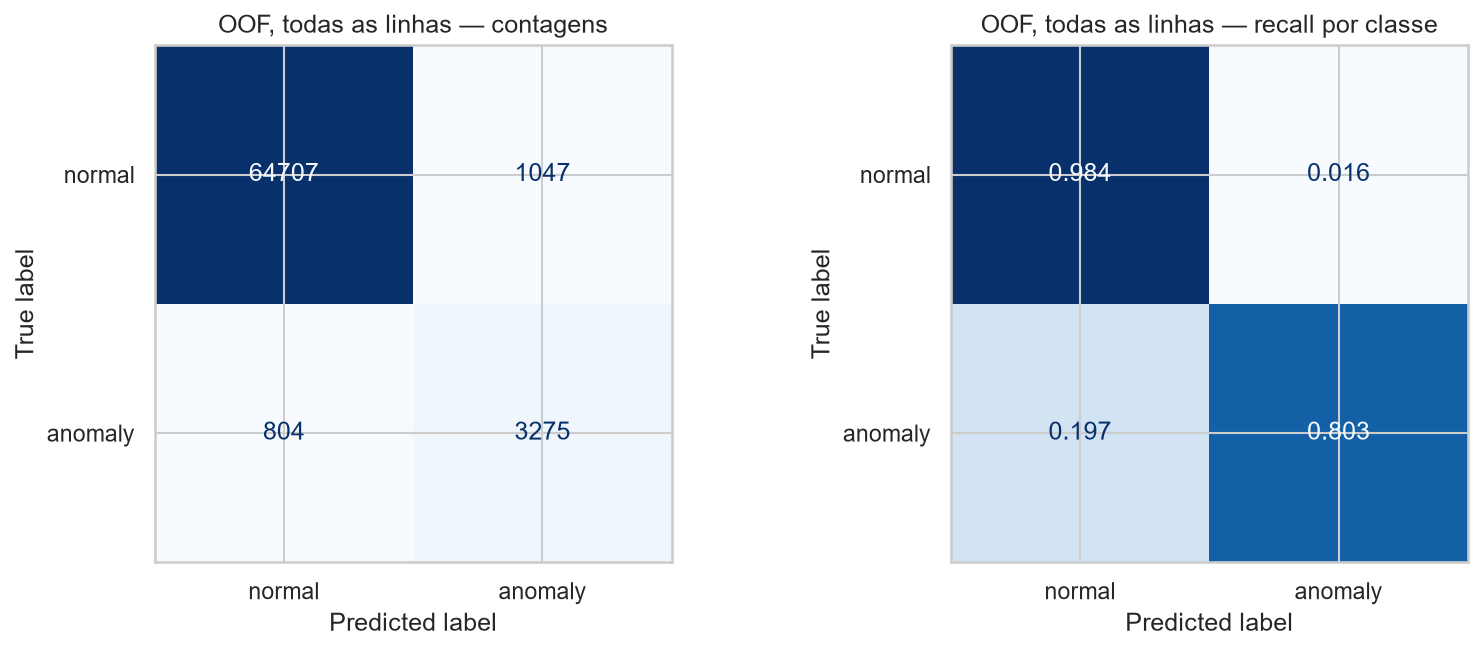
\includegraphics[width=\linewidth,height=0.26\textheight,keepaspectratio]{figuras/mod_confusao_oof.png}
\caption{Matriz de confusão das previsões fora do fold, em todas as linhas. À esquerda, as contagens; à direita, a proporção de acertos por classe.}
\end{figure}

\begin{itemize}
\item \textbf{Quase todo erro está nos conflitos.} Com o limiar escolhido no OOF (0,03), o F1-macro em todas as linhas é 0,8828. O modelo erra 1.851 linhas, e 1.706 delas estão entre as 3.730 linhas com rótulo contraditório: nesses grupos, a mesma linha tem os dois rótulos e recebe uma só previsão. No resto da base (66.103 linhas), ele erra 145 e o F1-macro é 0,983.
\item \textbf{Fora dos conflitos, o modelo deixa passar 3,7\% dos ataques} (81 de 2.183) e dá alarme falso em 0,1\% das conexões normais (64 de 63.920).
\item \textbf{Os ataques perdidos se parecem com tráfego normal.} 60 dos 81 têm \texttt{flag=SF}, que indica uma conexão encerrada normalmente. Essa flag aparece em 95\% do tráfego normal e em só 21\% dos ataques. Eles se concentram em serviços de login e transferência de arquivos (\texttt{private}, \texttt{ftp\_data}, \texttt{telnet}, \texttt{http}). Isso sugere ataques de acesso remoto, que não deixam rastro nas estatísticas de tráfego e são justamente os mais difíceis de detectar no KDD.
\item \textbf{O serviço \texttt{private} concentra também os alarmes falsos} (31 dos 64). Nesse serviço, as duas classes se sobrepõem.
\end{itemize}

\begin{figure}[H]
\centering
\begin{minipage}{0.49\linewidth}
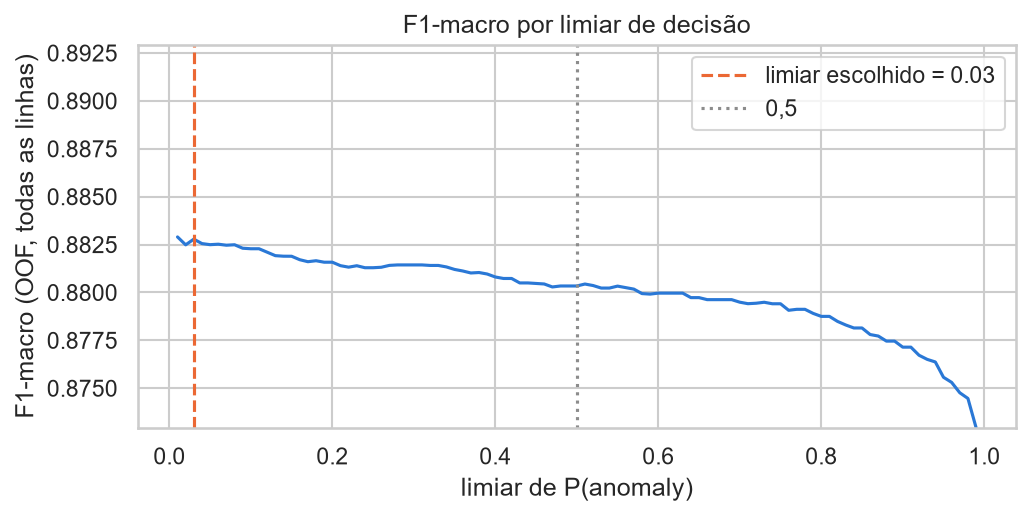
\includegraphics[width=\linewidth]{figuras/mod_limiar.png}
\end{minipage}\hfill
\begin{minipage}{0.49\linewidth}
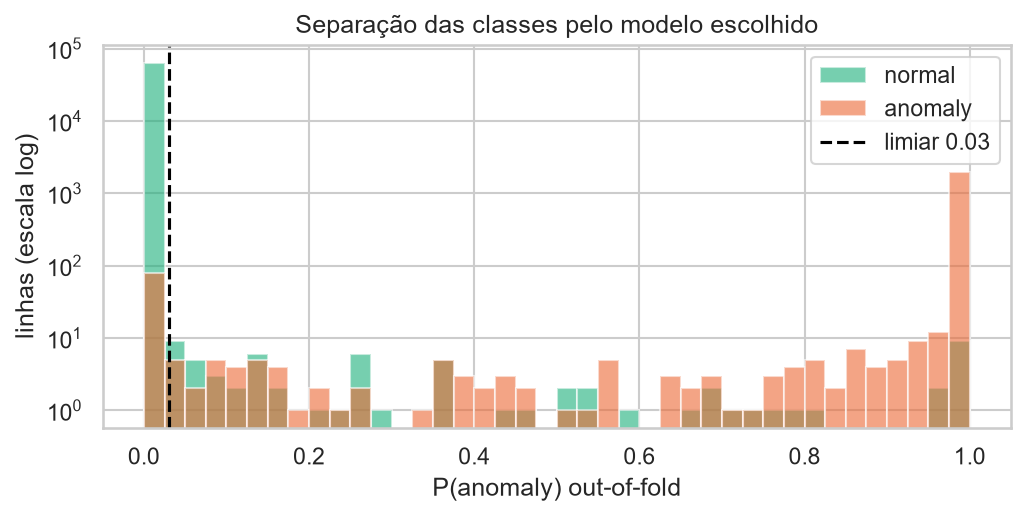
\includegraphics[width=\linewidth]{figuras/mod_probabilidades.png}
\end{minipage}
\caption{À esquerda, o F1-macro em função do limiar de decisão. À direita, a distribuição das probabilidades previstas por classe.}
\end{figure}

\begin{itemize}
\item \textbf{O limiar exato pesa pouco.} O F1-macro fica a menos de 0,002 do máximo para qualquer corte entre 0,01 e 0,39; em 0,5 ele cai só para 0,8803. O limiar escolhido é baixo por causa dos conflitos: nos 1.376 grupos com o mesmo número de cópias de cada rótulo, prever \texttt{anomaly} rende mais F1-macro do que prever \texttt{normal}, porque cada acerto na classe rara pesa mais.
\item \textbf{O modelo é confiante na grande maioria das linhas.} Quase todas as probabilidades estão perto de 0 ou de 1. Fora dos conflitos, os erros ficam numa faixa estreita de exemplos ambíguos. Isso explica por que as votações não ajudaram: esses exemplos não são erros aleatórios de um modelo, são casos que os 41 atributos não conseguem separar.
\end{itemize}

% =====================================================================
\section{Escolha e congelamento do modelo final}

\textbf{Decisão: HGB da busca ampliada.} Aplicando a regra da Seção~1, a votação HGB + XGBoost + RF tem a maior média, mas o HGB fica a 0,0007 dela, quatro vezes menos que o desvio entre folds. Os dois estão empatados, e o empate vai para o mais simples. O HGB:
\begin{itemize}
\item é um único modelo, visto na disciplina, sem passos extras;
\item treina em cerca de 1/9 do tempo da votação tripla;
\item pode ser explicado diretamente na Etapa 4;
\item tem a maior média entre os modelos únicos empatados (0,8819, contra 0,8815 do LightGBM e 0,8812 do RF).
\end{itemize}

Resumindo: \emph{todos os candidatos de boosting ficam perto de 0,882 e são equivalentes dentro do ruído; escolhemos o mais simples.}

\textbf{Um cuidado honesto.} O ganho do HGB da busca ampliada sobre o da primeira busca (0,8819 contra 0,8811) também está dentro do ruído. Além disso, a busca usou a mesma divisão de folds da semente 42 que entra na validação 3$\times$5, o que dá a ele uma leve vantagem otimista. Como os dois são o mesmo algoritmo, com pipeline idêntico, isso não muda a conclusão.

A configuração final foi gravada em \texttt{results/final\_config.json}:

\begin{table}[H]
\centering
\caption{Configuração congelada do modelo final.}
\begin{adjustbox}{max width=\linewidth}
\begin{tabular}{ll}
\toprule
Item & Valor \\
\midrule
Algoritmo & \texttt{HistGradientBoostingClassifier}, com categorias e NaN nativos \\
Hiperparâmetros & \texttt{learning\_rate=0.08}, \texttt{max\_iter=500}, \texttt{max\_leaf\_nodes=63}, \texttt{min\_samples\_leaf=20}, \texttt{max\_features=0.7}, \texttt{l2\_regularization=0.0} \\
Pré-processamento & remoção dos grupos com rótulo contraditório no treino (\texttt{drop\_inconsistent}); valores impossíveis viram NaN; sem imputação, escala nem balanceamento \\
Atributos & os 41 atributos de rede, sem colunas de vazamento nem derivadas \\
Limiar de decisão & escolhido pelo \texttt{ThresholdClassifier} com previsões fora do fold no próprio treino (média de 0,04 na validação) \\
F1-macro esperado & \textbf{0,8819 $\pm$ 0,0030} (CV agrupada 3$\times$5, todas as linhas, como a métrica oficial) \\
Contraste sem conflitos & 0,9817 (mesmo modelo, só linhas únicas e sem rótulo contraditório) \\
Congelado em & 24/11/2026 (refeito com a métrica corrigida), versão da base \texttt{db8fb3ac} \\
\bottomrule
\end{tabular}
\end{adjustbox}
\end{table}

Para garantir que o arquivo descreve exatamente o modelo avaliado, o notebook reconstrói o pipeline a partir do JSON e confirma que ele gera a mesma chave registrada na validação. A partir deste ponto, nenhuma escolha das Etapas 2 e 3 muda.

% =====================================================================
\section{Conclusões e próximos passos}

\begin{table}[H]
\centering
\caption{Resumo da Etapa 3.}
\begin{adjustbox}{max width=\linewidth}
\begin{tabular}{p{4.2cm}p{11.6cm}}
\toprule
Pergunta & Resposta \\
\midrule
Melhor família & boosting de árvores (HGB e LightGBM empatados), com Random Forest e as votações no empate \\
Modelo final & HGB com categorias e NaN nativos, limpeza de rótulos e limiar ajustado \\
F1-macro esperado & 0,8819 $\pm$ 0,0030 na validação agrupada 3$\times$5, em todas as linhas (teto teórico 0,905; sem conflitos, 0,9817) \\
O que mais rendeu & limpeza de rótulos no boosting (Etapa 2) e ajuste do limiar de decisão \\
O que não rendeu & balanceamento, redução, votações, média de sementes, atributos novos, CatBoost e o ajuste de hiperparâmetros \\
Erros restantes & 92\% estão nas linhas com rótulo contraditório; os demais são, em sua maioria, ataques com \texttt{flag=SF} que imitam conexões normais \\
\bottomrule
\end{tabular}
\end{adjustbox}
\end{table}

\textbf{O preço de não vazar.} As colunas de vazamento, sozinhas, chegariam a 0,889 de F1-macro na mesma métrica (Etapa 1), acima de qualquer modelo de tráfego. Abrimos mão delas porque são registradas depois do evento (alertas e tempo de resposta do analista) e não existiriam no momento de classificar uma conexão real.

\textbf{O que esperar do teste.} A professora calcula o F1-macro em \emph{todas} as linhas do teste, como a nossa validação. Se o teste tiver cópias e rótulos contraditórios na mesma proporção do treino, a nota oficial deve ficar perto de 0,88. Se tiver menos conflitos, pode ficar acima, até perto do valor sem conflitos (0,98). O ruído vale para todas as equipes e não muda a ordem entre os modelos.

\textbf{Próximo passo (Etapa 4).} O notebook 04 vai ler o \texttt{final\_config.json}, treinar o modelo no treino inteiro, abrir o teste uma única vez, gerar o arquivo de submissão e registrar a sua assinatura SHA-256. Depois, vamos explicar as decisões do modelo (importância dos atributos e SHAP).

\subsection*{Auditoria de vazamento}

A auditoria automática do projeto (\texttt{python -m nslkdd.audit notebooks/03\_modelagem.ipynb}) retornou \textbf{0 achados e 0 erros}. Nenhuma célula carrega o teste, junta treino e teste ou ajusta transformações fora do pipeline. Os atributos novos da Seção~4 são calculados por uma fórmula fixa, linha a linha, verificada por testes automáticos (\texttt{tests/test\_leakage.py}), e o limiar de decisão é sempre escolhido com previsões feitas fora do fold.

\section*{Declaração de uso de Inteligência Artificial}
\addcontentsline{toc}{section}{Declaração de uso de Inteligência Artificial}

Declaramos que a ferramenta de Inteligência Artificial Claude
foi utilizada como apoio à revisão crítica das análises e
dos procedimentos desenvolvidos pela equipe, bem como à
formatação e ao aprimoramento da redação deste relatório,
com o objetivo de verificar a consistência do trabalho
realizado e melhorar a clareza, a organização e a
apresentação textual das informações.

\end{document}
